Consider the following MDP, with two states $B$ and $C$, with 1 action in state $B$ and two actions in state $C$, with $\gamma = 1.0$.
Assume the action values are initialized, for all state-action pairs, $Q(s,a) = 0$.
\begin{enumerate}
\item What is the optimal policy for this MDP and what are the optimal action-values $q^{*}(s,a)$?
\item What policy is executed by being greedy with the initialized action-values?
\item Imagine you got to interact with the environment for one episode, and observed the episode $\{S_0 = B, A_0 = 1, R_1 = 1, S_1 = C, A_1 = 1, R_2 = 1$. This episode consists of two transitions, what is the SARSA update for both transitions?
\item For the transitions in the previous question, what is the Q-learning update?
\item If you see the same transitions again, how will the update change for SARSA and for Q-learning?
\end{enumerate}
\begin{figure}[h!]
  \center
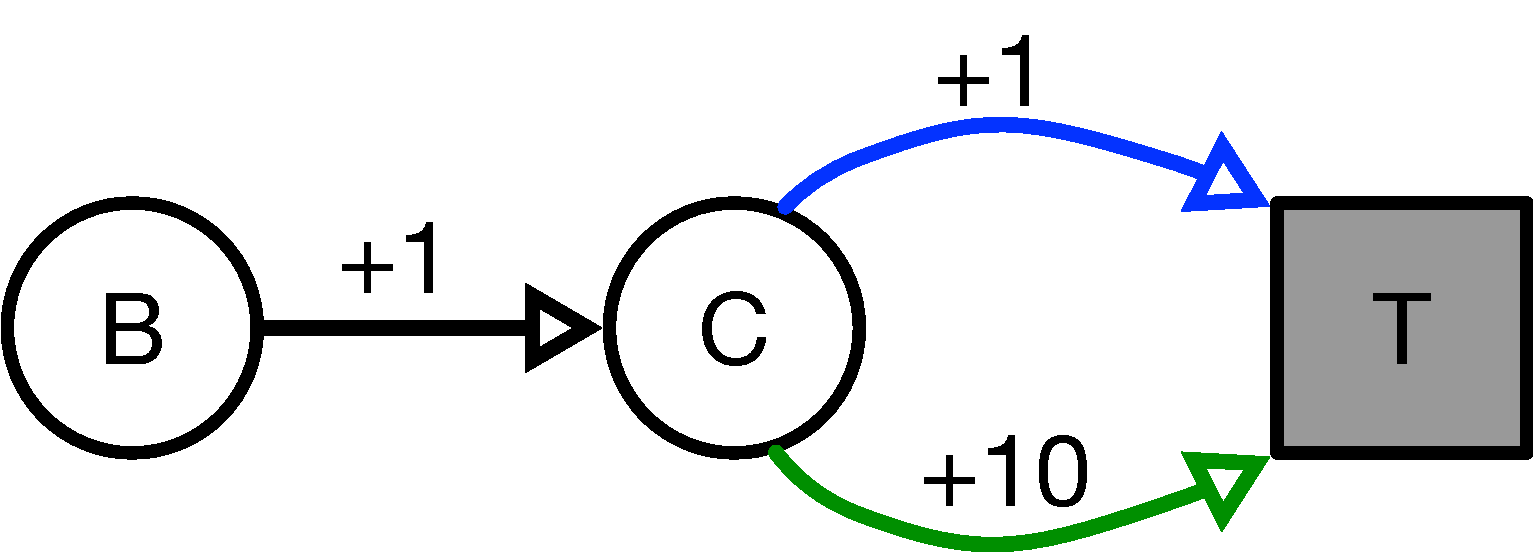
\includegraphics[width=0.5\linewidth]{figures/c2_2state.pdf}
\end{figure}

